\documentclass[a4paper]{report}

\usepackage{graphicx}
\usepackage{float}
\usepackage{hyperref}
\usepackage{xcolor}
\usepackage[spanish]{babel}
\usepackage{listings}
\usepackage{enumitem}
\usepackage[utf8]{inputenc}

\lstset{language=bash, frame=tlrb, basicstyle=\scriptsize, breaklines=true, numberbychapter=false,numbers=left}
\setlist[enumerate]{noitemsep}
\setlist[itemize]{noitemsep}

\begin{document}

\title{Universidad Nacional de La Plata\\Facultad de Informática\\ \bigskip
  Especialización en Cómputo de Altas Prestaciones\\ \bigskip
  Herramientas para el Soporte de Análisis de Rendimiento}

\author{
  Alumno: Andrés More - {\tt amore@hal.famaf.unc.edu.ar}\\
  Director: Dr Fernando G. Tinetti - {\tt fernando@lidi.info.unlp.edu.ar}
}

\date{Octubre de 2013}

\maketitle

\begin{abstract}

 Este documento describe una investigación realizada como trabajo final para la Especialización en Cómputo de Altas Prestaciones dictada en la Facultad de Informática de la Universidad Nacional de La Plata. El tema de investigación consiste en métodos y herramientas para el análisis del comportamiento de aplicaciones de alto rendimiento.

  \bigskip

  Luego de la introducción de terminología y bases teóricas del análisis cuantitativo de rendimiento, se resume la experiencia de utilizar herramientas para conocer donde se debería localizar los esfuerzos de optimización.

  \bigskip

  Este trabajo resume la experiencia que debe atravesar cualquier
  individuo en busca de las diferentes alternativas para el análisis de
  rendimiento; incluyendo la selección de herramientas de soporte y la
  definición de un procedimiento sistemático para la aplicación iterativa
  de las mismas.

  \bigskip

  Este trabajo contribuye entonces con un resumen de las teoría del análisis del
  rendimiento más una descripción de los herramientas de soporte 
  disponibles en el momento. Se propone también un proceso para analizar el
  rendimiento, ejemplificando su aplicación a un conjunto de núcleos de
  cómputo no triviales.

\end{abstract}

\tableofcontents

\chapter{Introducción}

Este capítulo introduce este trabajo y su alcance. Luego de revisar la
motivación de esta investigación, se resume el estado actual del análisis
del rendimiento y se detalla el contenido restante del informe.

\section{Motivación}

En el área de cómputo de altas prestaciones los desarrolladores son los mismos
especialistas del dominio del problema a resolver. Las rutinas
más demandantes de cálculo son en su mayoría científicas y su
alta complejidad hace posible su correcta implementación sólo por los mismos investigadores.
Este hecho resulta en un tiempo reducido de análisis de resultados
e impacta directamente en la productividad de los grupos de investigación y
desarrollo.

\bigskip

Con mayor impacto que en otras áreas de la computación, el código
optimizado correctamente puede ejecutarse órdenes de magnitud mejor que una implementación
directa \cite{mm-matrixmultiplicationtool}. Además, se utiliza
programación en paralelo para obtener una mejor utilización de la
capacidad de cómputo disponible; aumentando por lo tanto la complejidad de
implementación, depuración y optimización \cite{parallel-programming}.

\bigskip

Frecuentemente el proceso de optimización termina siendo
hecho de modo {\it ad-hoc}, sin conocimiento pleno de las herramientas disponibles y
sus capacidades, y sin la utilización de información cuantitativa para dirigir los
esfuerzos de optimización. Es incluso frecuente la implementación directa
de algoritmos en lugar de la utilización de librerías ya disponibles, optimizadas
profundamente y con correctitud comprobada.

\section{Alcance}

Este trabajo considera en particular a los sistemas de memoria distribuida corriendo sobre
GNU/Linux, denominados sistemas Beowulf \cite{beowulf}. A través de las
estadísticas mostradas por el Top500 \footnote{El Top500 es una lista actualizada de super-computadoras
de acuerdo al benchmark Linpack, disponible en {\tt http://www.top500.org}.}, se
puede determinar que son los más utilizados en el cómputo de aplicaciones de alto rendimiento en la actualidad.

\section{Estado Actual}

Actualmente existen numerosas y diversas herramientas para el análisis de rendimiento.
Estas funcionan a diferentes niveles de abstracción: desde contadores de eventos
a nivel de {\it hardware}, pasando por monitores de recursos dentro del núcleo del sistema operativo,
instrumentación automática de código, y hasta la simple utilización del tiempo de ejecución 
de una aplicación o la comparación contra un trabajo sintético de referencia.

\bigskip

Ademas de teoría de análisis del rendimiento, un desarrollador necesita
conocer de las herramientas listadas en la tabla \ref{table:tools}.

\begin{table}[H]
    \caption{Herramientas de Soporte para Optimización}
    \centering
    \begin{tabular}{|l|l|}\hline
      {\bf Herramienta} & {\bf Descripción} \\ \hline
      gprof & Muestra información de perfil de llamadas a funciones \\ \hline
      oprofile & Muestra información de perfil de sistema \\ \hline
      stream & Benchmark de jerarquía de memoria \\ \hline
      hpl & Benchmark de capacidad de cómputo \\ \hline
      imb pingpong & Benchmark de latencia y ancho de banda \\ \hline
      hpcc & Conjunto de benchmarks \\ \hline
    \end{tabular}
    \label{table:tools}
\end{table}

\section{Organización del Contenido}

El resto del documento explica teoría introductoria sobre el análisis del rendimiento, que luego es
aplicada a través del resto del documento.

\bigskip

El capítulo 2 discute el análisis de rendimiento, sus
principios y teoría. El capítulo 3 detalla las herramientas más
utilizadas. El capítulo 4 ejemplifica la aplicación de las herramientas
para obtener información de análisis a través de un proceso sistemático.
El capítulo 5 concluye y el capítulo 6 detalla posibles extensiones de este trabajo.

\chapter{Análisis de Rendimiento}

Este capítulo introduce el concepto de rendimiento y teoría básica sobre su análisis.
Se revisa la utilización de pruebas de referencia como práctica recomendada.

\section{Definición}

El rendimiento se caracteriza por la cantidad de trabajo de cómputo que se
logra en comparación con la cantidad de tiempo y los recursos ocupados.
El rendimiento debe ser evaluado entonces de forma cuantificable, utilizando alguna
métrica en particular de modo de poder comparar relativamente dos sistemas o
el comportamiento de un mismo sistema bajo una configuración distinta.

\section{Métricas}

Algunos ejemplos de medida de rendimiento son:

\begin{enumerate}
\item el ancho de banda y la latencia mínima de un canal de comunicación,
  una jerarquía de memorias o de la unidad de almacenamiento.
\item la cantidad de instrucciones, operaciones, datos o trabajo procesado
  por cierta unidad de tiempo.
\item rendimiento asociado al costo del equipamiento, incluyendo mantenimiento
 periódico, personal dedicado y gastos propios del uso cotidiano.
\item rendimiento por unidad de energía consumida (electricidad).

\end{enumerate}

Un método de medición de rendimiento indirecto consiste en medir el uso de
los recursos del sistema mientras se ejercita el mismo con un trabajo dado.
Por ejemplo: el nivel de carga de trabajo en el sistema, la cantidad de operaciones realizadas por el
sistema operativo o la unidad de procesamiento, la utilización de memoria o
archivos temporales e incluso el ancho de banda de red utilizado durante la comunicación.

\section{Técnicas de Análisis}

El procedimiento de mejora general usualmente consiste en ciclos iterativos de medir, localizar, optimizar,
comparar (Figura \ref{fig:cycle}). Es muy importante mantener la disciplina en realizar un cambio a la
vez ya que esto asegura resultados reproducibles y convergentes, sin efectos no deseados.

\begin{figure}[H]
\begin{center}
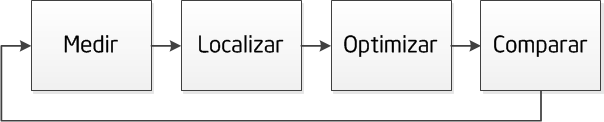
\includegraphics[width=10cm]{cycle.png}
\caption{Análisis Iterativo}
\label{fig:cycle}
\end{center}
\end{figure}

A la hora de tomar decisiones, éstas deben estar basadas en datos concretos, ya que en caso contrario se podría estar trabajando en lugares donde no se va a obtener un rédito adecuado.

\bigskip

En el caso de tener problemas de desviación en los resultados medidos, es aconsejable obtener un gran número de muestras y utilizar un valor promedio para asegurarse de evitar errores de medición tanto como sea posible. También es preferible aumentar el tamaño del problema a resolver, o la definición de los resultados para ejercitar por más tiempo y tener así un resultado más estable.
Suponiendo una distribución normal de resultados, se suelen controlar que haya menos de 3 $ \sigma $ de diferencia. Se busca que la mayoría de los resultados queden cerca de su promedio, como muestra la Figura \ref{fig:deviation}.

\begin{figure}[H]
\label{fig:deviation}
\begin{center}
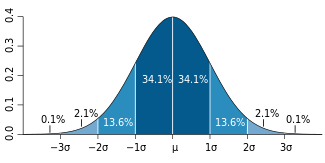
\includegraphics[width=10cm]{deviation.png}
\caption{Desviación Normal}
\end{center}
\end{figure}

Los resultados deben también ser correctamente guardados para evitar
problemas de datos. Si la configuración del sistema es dinámica entonces la
reproducción de resultados es no trivial. En el caso de no tener una
configuración de sistema estable en el tiempo, es recomendable siempre
ejecutar una versión optimizada contra una versión de referencia en un mismo
sistema de cómputo.

\bigskip

Para comparar se recomienda utilizar la media geométrica según la ecuación \ref{eq:geomean} en lugar de la aritmética, ya que permite dimensionar la tendencia central de un valor típico en un conjunto
de números. Esto permite reducir el impacto de ruido introducido por una ejecución
problemática.

\begin{equation}
\label{eq:geomean}
G = \sqrt[n]{x_{1} \ldots x_{n}}
\end{equation}

Esta cuenta puede ser muy costosa y requerir de una alta precisión, por lo que se
suele tomar el anti-logaritmo del promedio de los logaritmos de los valores siguiendo
la ecuación \ref{eq:geomean-log}.

\begin{equation}
\label{eq:geomean-log}
G = 10 ^{( log _{10} (x_{1}) + \ldots + log _{10} (x_{n}) ) / n}
\end{equation}

\bigskip

\section{Pruebas de Rendimiento}

Para medir el rendimiento se utilizan pruebas de referencia denominadas {\em benchmarks}; éstas pueden ser aplicaciones sintéticas construídas especialmente para ejercitar ciertos recursos computacionales, o bien
aplicaciones del mundo real ejecutadas sobre un conjunto de datos prefijado.

\bigskip

Al tener valores de referencia se pueden caracterizar los sistemas de modo de predecir el rendimiento de una aplicación.
Los valores a los que se llegan con un {\it benchmark} suelen ser más prácticos y
comparables que los teóricos de acuerdo a condiciones ideales de uso de recursos.
También es posible garantizar que el sistema sigue en un mismo estado con el correr\
del tiempo y después de cambios de configuraciones en {\it hardware} o {\it software}.

\bigskip

Las características deseables en un {\it benchmark} son portabilidad, simplicidad, estabilidad y
reproducción de resultados. Esto permite que sean utilizadas para realizar
mediciones cuantitativas y así realizar comparaciones de optimizaciones o
entre sistemas de cómputo diferentes. También se pide que el tiempo de
ejecución sea razonable y que el tamaño del problema sea ajustable para
poder mantener su utilidad con el paso del tiempo y el avance de las
tecnologías.

\bigskip

A continuación se introducen algunas de las más utilizadas para cómputo
de altas prestaciones (listadas en la tabla \ref{table:benchmark-list}),
y posteriormente algunos detalles específicos e instancias
de sus datos de salida para ser utilizados a manera de ejemplo.

\begin{table}[H]
    \caption{Benchmarks}
    \begin{center}
    \begin{tabular}{|l|l|l|}\hline
      {\bf Benchmark} & {\bf Componente} & {\bf Descripción} \\ \hline
      STREAM & Memoria & Ancho de banda sostenido \\ \hline
      Linpack & Procesador & Operaciones de punto flotante \\ \hline
      IMB Ping Pong & Red & Latencia y ancho de banda de comunicación \\ \hline
      HPCC & Sistema & Múltiples componentes \\ \hline
        \end{tabular}
  \label{table:benchmark-list}
  \end{center}
\end{table}

\bigskip

Los {\it benchmarks} pueden ser utilizados para diferentes propósitos. Primero,
los valores reportados son usados como referencia para contrastar rendimiento.
Segundo, su desviación demuestra que algo ha cambiado en el sistema (por lo tanto
su no desviación indica que el sistema sigue saludable). Por último,
un {\it benchmark} sintético implementando el cómputo que uno quiere realizar
muestra el rendimiento máximo posible a obtener en la práctica.

\subsection{STREAM}

STREAM \cite{stream} es un {\it benchmark} sintético a través de un simple
programa que mide el ancho de banda de memoria sostenido en MB/s y el
rendimiento de computación relativa de algunos vectores simples de cálculo.
Se utiliza para dimensionar el ancho de banda de acceso de escritura o lectura
a la jerarquía de memoria principal del sistema bajo análisis.

\bigskip

Dentro de una misma ejecución de este {\it benchmark} se ejercitan diferentes
operaciones en memoria, listadas en la tabla \ref{table:stream}.

\begin{table}[H]
\caption{Operaciones del Benchmark STREAM}
  \begin{center}
    \begin{tabular}{|l|l|l|}\hline
      {\bf Función} & {\bf Operación} & {\bf Descripción} \\ \hline
      copy & $ \forall i $ $ b_{i} = a_{i} $ & Copia simple \\ \hline
      scale & $ \forall i $ $ b_{i} = c \times a_{i} $ & Multiplicación escalar \\ \hline
      add & $ \forall i $ $ c_{i} = b_{i} + a_{i} $ & Suma directa \\ \hline
      triad & $ \forall i $ $ c_{i} = b_{i} + c \times a_{i} $ & Suma y multiplicación escalar \\ \hline
    \end{tabular} 
   \end{center}
 \label{table:stream}
\end{table}

La salida en pantalla muestra entonces los diferentes tiempos conseguidos y la cantidad de información transferida por unidad de tiempo.
Como último paso, el programa valida también la solución computada.

{\small
\begin{verbatim}
  STREAM version $Revision: 1.2 $
  -------------------------------------------------------------
  This system uses 8 bytes per DOUBLE PRECISION word.
  -------------------------------------------------------------
  Array size = 10000000, Offset = 0
  Total memory required = 228.9 MB.
  Each test is run 10 times, but only the *best* time is used.
  -------------------------------------------------------------
  Function     Rate (MB/s)   Avg time     Min time     Max time
  Copy:        4764.1905       0.0337       0.0336       0.0340
  Scale:       4760.2029       0.0338       0.0336       0.0340
  Add:         4993.8631       0.0488       0.0481       0.0503
  Triad:       5051.5778       0.0488       0.0475       0.0500
  -------------------------------------------------------------
  Solution Validates
\end{verbatim}
}

\subsection{Linpack}

Linpack \cite{linpack} es un conjunto de subrutinas {\it FORTRAN} que resuelven
problemas de álgebra lineal como ecuaciones lineales y multiplicación de
matrices. High Performance Linpack (HPL) \cite{hpl} es una versión portable del {\it benchmark} que incluye
el paquete Linpack pero modificado para sistemas de memoria distribuida.

\bigskip

Este {\it benchmark} es utilizado mundialmente para la comparación de la
velocidad de las supercomputadoras en el ranking TOP500. 
Un gráfico del TOP500 de los últimos años demuestra claramente la
tendencia en crecimiento de rendimiento; también la relación entre el primero,
el último y la suma de todos los sistemas en la lista.

\begin{figure}[H]
\begin{center}
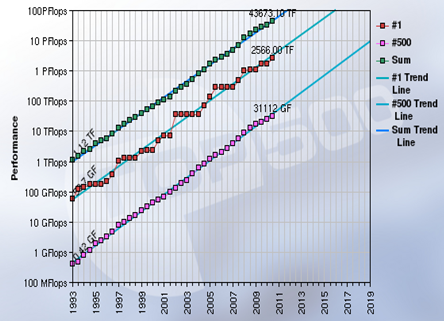
\includegraphics[width=10cm]{top500.png}
\caption{Indicadores Históricos del Top500}
\end{center}
\end{figure}

Este {\it benchmark} requiere conocimiento avanzado para una correcta configuración,
por ejemplo el tamaño de bloque que se va a utilizar para la distribución de trabajo
debe estar directamente relacionado con el tamaño del {\it cache} de memoria del procesador.

\bigskip

La salida en pantalla resume entonces los datos de entrada y los resultados conseguidos.
Como último paso el programa valida que los resultados sean correctos.

{\small
\begin{verbatim}
=================================================================
HPLinpack 2.0 - High-Performance Linpack benchmark - Sep 10, 2008
Written by A. Petitet and R. Clint Whaley
============================================================
The following parameter values will be used:
N      :   28888
NB     :     168
PMAP   : Row-major process mapping
P      :       4
Q      :       4
PFACT  :   Right
NBMIN  :       4
NDIV   :       2
RFACT  :   Crout
BCAST  :  1ringM
DEPTH  :       0
SWAP   : Mix (threshold = 64)
L1     : transposed form
U      : transposed form
EQUIL  : yes
ALIGN  : 8 double precision words
-------------------------------------------------------------------------------
- The matrix A is randomly generated for each test.
- The relative machine precision (eps) is taken to be 1.110223e-16
- Computational tests pass if scaled residuals are less than 16.0

Column=000168 Fraction=0.005 Mflops=133122.97
...
Column=025872 Fraction=0.895 Mflops=98107.60
==========================================================================
T/V                N   NB   P    Q             Time                 Gflops
WR01C2R4       28888  168   4    4           165.83              9.693e+01
--------------------------------------------------------------------------
||Ax-b||_oo/(eps*(||A||_oo*||x||_oo+||b||_oo)*N) = 0.0043035 ...... PASSED
==========================================================================
Finished      1 tests with the following results:
1 tests completed and passed residual checks,
0 tests completed and failed residual checks,
0 tests skipped because of illegal input values.
\end{verbatim}
}

\bigskip

Existe cierta controversia de que no es una buena forma de ejercitar un
sistema de cómputo distribuido ya que no implica uso significativo de la
red, sólo procesamiento intensivo de aritmética de punto flotante
sobre la jerarquía local de memoria.

\subsection{Intel MPI Benchmarks}

Es un conjunto de {\it benchmarks} cuyo objetivo es ejercitar las funciones
más importantes del estándar para librerías de paso de mensajes (MPI, por sus siglas en inglés) \cite{mpi}.
El más conocido es el popular ping-pong, el cual ejercita la transmisión de mensajes ida y vuelta entre dos nodos de
cómputo con diferentes tamaños de mensajes. \cite{latency}.

\bigskip

Para obtener el máximo ancho de banda disponible, se ejercita la comunicación a través de mensajes con datos grandes. Para obtener la mínima latencia, se ejercita la comunicación con mensajes vacíos, es decir transmitiendo mensajes sin dato alguno.

{\small
\begin{verbatim}
# Intel (R) MPI Benchmark Suite V3.1, MPI-1 part
# Date                  : Wed Mar  3 10:45:16 2010
# Machine               : x86_64
# System                : Linux
# Release               : 2.6.16.46-0.12-smp
# Version               : #1 SMP Thu May 17 14:00:09 UTC 2007
# MPI Version           : 2.0
# MPI Thread Environment: MPI_THREAD_SINGLE
# Calling sequence was: ../IMB-MPI1 pingpong
# Minimum message length in bytes:   0
# Maximum message length in bytes:   4194304
#
# MPI_Datatype                   :   MPI_BYTE
# MPI_Datatype for reductions    :   MPI_FLOAT
# MPI_Op                         :   MPI_SUM
#
# List of Benchmarks to run: PingPong
#---------------------------------------------------
# Benchmarking PingPong
# #processes = 2
#---------------------------------------------------
#bytes     #repetitions  t[usec]     Mbytes/sec
0              1000           17.13        0.00
1              1000           17.89        0.05
2              1000           17.82        0.11
4              1000           17.95        0.21
...
1048576    40              8993.23    111.19
2097152    20              17919.20  111.61
4194304    10              35766.45  111.84
\end{verbatim}
}

\subsection{HPC Challenge}

El {\it benchmark} HPC Challenge \cite{hpcc} (HPCC) está compuesto internamente por un conjunto de
varios núcleos de cómputo: entre ellos STREAM, HPL, Ping Pong, Transformadas de {\it Fourier}
y otros ejercitando la red de comunicación.

\bigskip

Este benchmark muestra diferentes resultados que son representativos
y puestos en consideración de acuerdo al tipo de aplicación en discusión.
La mejor máquina depende de la aplicación específica a ejecutar, ya que algunas
aplicaciones necesitan mejor ancho de banda de memoria, mejor canal de comunicación, o
o simplemente la mayor capacidad de cómputo de operaciones flotantes posible.

\bigskip

Una analogía interesante para entender como el {\it benchmark} se relaciona a diferentes núcleos de cómputo
se muestra en la figura \ref{fig:locality}. Por ejemplo al tener un problema que
utiliza principalmente acceso a memoria local, se puede suponer que un sistema con
buenos resultados de STREAM va ser útil.

\bigskip

\begin{figure}[H]
\begin{center}
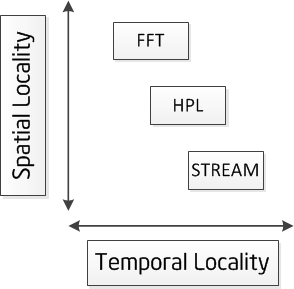
\includegraphics[width=10cm]{locality.png}
\caption{Localidad}
\label{fig:locality}
\end{center}
\end{figure}

\bigskip

Para una mejor comparación de resultados de HPCC se utilizan diagramas
denominados {\it kiviats}, se muestra un ejemplo en la figura \ref{fig:kiviat}.
Se comparan entonces dos sistemas, uno con mejor rendimiento que el otro.

\begin{figure}[H]
\begin{center}
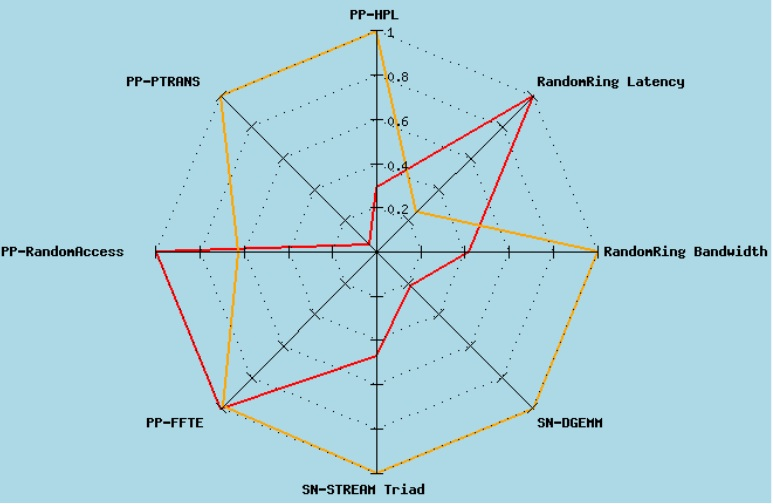
\includegraphics[width=10cm]{kiviat.png}
\caption{Diagrama Kiviat}
\label{fig:kiviat}
\end{center}
\end{figure}

Un ejemplo de la salida que se muestra durante la ejecución se muestra a continuación.

{\small

\begin{verbatim}
This is the DARPA/DOE HPC Challenge Benchmark version 1.2.0 October 2003
Produced by Jack Dongarra and Piotr Luszczek
Innovative Computing Laboratory
University of Tennessee Knoxville and Oak Ridge National Laboratory
See the source files for authors of specific codes.
Begin of Summary section.
\end{verbatim}

\begin{minipage}[b]{0.5\linewidth}
\begin{verbatim}
VersionMajor=1
VersionMinor=2
LANG=C
Success=1
CommWorldProcs=3
MPI_Wtick=1.000000e-06
HPL_Tflops=0.0674008
HPL_time=26.3165
HPL_eps=1.11022e-16
HPL_N=13856
HPL_NB=64
HPL_nprow=1
HPL_npcol=3
HPL_depth=2
HPL_nbdiv=2
HPL_nbmin=8
HPL_cpfact=C
HPL_crfact=R
HPL_ctop=1
HPL_order=R
dweps=1.110223e-16
sweps=5.960464e-08
HPLMaxProcs=3
HPLMinProcs=3
DGEMM_N=4618
StarDGEMM_Gflops=68.9053
SingleDGEMM_Gflops=70.2692
PTRANS_GBs=0.794254
PTRANS_time=0.479293
PTRANS_residual=0
PTRANS_n=6928
PTRANS_nb=64
PTRANS_nprow=1
PTRANS_npcol=3
MPIRandomAccess_N=134217728
MPIRandomAccess_time=30.4475
MPIRandomAccess_CheckTime=14.0705
MPIRandomAccess_Errors=0
\end{verbatim}
\end{minipage}
\hspace{0.5cm}
\begin{minipage}[b]{0.5\linewidth}
\begin{verbatim}
MPIRandomAccess_ErrorsFraction=0
MPIRandomAccess_ExeUpdates=536870912
MPIRandomAccess_GUPs=0.0176327
MPIRandomAccess_TimeBound=-1
MPIRandomAccess_Algorithm=0
RandomAccess_N=33554432
StarRandomAccess_GUPs=0.0186362
SingleRandomAccess_GUPs=0.0184568
STREAM_VectorSize=21332081
STREAM_Threads=8
StarSTREAM_Copy=4.34705
StarSTREAM_Scale=3.24366
StarSTREAM_Add=3.41196
StarSTREAM_Triad=3.46198
SingleSTREAM_Copy=4.53628
SingleSTREAM_Scale=3.38984
SingleSTREAM_Add=3.59073
SingleSTREAM_Triad=3.65083
FFT_N=8388608
StarFFT_Gflops=2.17339
SingleFFT_Gflops=2.26806
MPIFFT_N=8388608
MPIFFT_Gflops=1.7043
MPIFFT_maxErr=1.77722e-15
MPIFFT_Procs=2
MaxPingPongLatency_usec=5.37932
RandomlyOrderedRingLatency_usec=5.70686
MinPingPongBandwidth_GBytes=0.675574
NaturallyOrderedRingBandwidth_GBytes=0.531278
RandomlyOrderedRingBandwidth_GBytes=0.529161
MinPingPongLatency_usec=5.24521
AvgPingPongLatency_usec=5.30978
MaxPingPongBandwidth_GBytes=0.682139
AvgPingPongBandwidth_GBytes=0.678212
NaturallyOrderedRingLatency_usec=5.79357
FFTEnblk=16
FFTEnp=8
FFTEl2size=1048576
\end{verbatim}
\end{minipage}

\begin{verbatim}
End of Summary section.
End of HPC Challenge tests.
\end{verbatim}
}

\section{Teoría}

Una vez obtenida una implementación eficiente, la única alternativa para mejorar el rendimiento es explotar el paralelismo que
ofrecen los sistemas de cómputo. Este paralelismo se puede explotar a diferentes niveles, desde instrucciones que ejecutan una misma operación a varios
datos a la vez (vectorización), pasando por la utilización de varias unidades de cómputo hasta la utilización de unidades de cómputo en diferentes sistemas para distribuir el trabajo.

\bigskip

El cálculo de las mejoras posibles de rendimiento, como priorizarlas y la estimación de su límite máximo es una tarea compleja.
Para ello existen algunas leyes frecuentemente utilizadas durante el análisis de rendimiento.

\subsection{Ley de {\it Amdahl}}

 La ley de {\it Amdahl} \cite{amdahl} dimensiona la mejora que puede obtenerse en un sistema de acuerdo a las mejoras logradas en sus
componentes. Nos ayuda a establecer un límite máximo de mejora y a estimar cuales pueden ser los resultados de mejora.

\bigskip

La mejora de un programa utilizando procesamiento múltiple en cómputo paralelo
está limitado por el tiempo necesario para completar su fracción serial o
secuencial. Frecuentemente el paralelismo solo afecta notoriamente cuando es
utilizado en un pequeño número de procesadores, o cuando se aplica a problemas
altamente escalables (embarrassingly parallel problems). Una vez paralelizado un
programa, los esfuerzos suelen ser enfocados en como minimizar
la parte secuencial, algunas veces haciendo más trabajo redundante pero en forma paralela.

\bigskip

La ley de {\it Amdahl} puede ser entonces modelada con la ecuación \ref{eq:amdahl}.

\begin{eqnarray}
\label{eq:amdahl}
S = \frac{1}{(1-P) + \frac{P}{N}}
\end{eqnarray}

donde $ P $ es el porcentaje de trabajo paralelizable ($ 1-P $ es entonces el trabajo en serie o secuencial), $ N $ es la cantidad de unidades de cómputo utilizadas.

\bigskip

Suponiendo que una aplicación requiere de un trabajo serial más un trabajo paralelizable; esta ley nos deja estimar la máxima ganancia posible
de modo que incluso teniendo infinitas unidades de cómputo la ganancia esta limitada como se muestra a continuación.

\begin{figure}[H]
\begin{center}
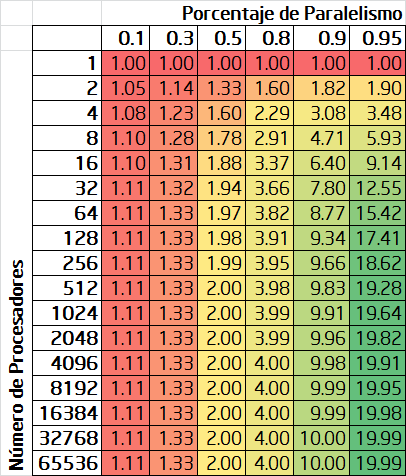
\includegraphics[width=7cm]{amdahl.png}
\caption{Mejora Máxima}
\label{fig:amdahl}
\end{center}
\end{figure}

La figura \ref{fig:amdahl} muestra que no importa la cantidad de unidades de
procesamiento que sean utilizadas, en el caso de tener solo un 10\% de paralelismo
en una aplicación, la mejora nunca va a superar 1.10x la original.
En el caso de tener un 95\%, la mejora no puede ser mejor a 20x.

\subsection{Ley de {\it Gustafson}}

Desde un punto de vista más general, la ley de {\it Gustafson}
\cite{gustafson} (computada mediante la ecuación \ref{eq:gustafson})
establece que las aplicaciones que manejan problemas
repetitivos con conjuntos de datos similares pueden ser fácilmente
paralelizadas. En comparación, la ley anterior no escala el tamaño o
resolución de problema cuando se incrementa la potencia de cálculo, es
decir asume un tamaño de problema fijo. 

\begin{eqnarray}
\label{eq:gustafson}
speedup(P) = P - \alpha \times ( P - 1)
\end{eqnarray}

donde $ P $ es el número de unidades de cómputo y $ \alpha $ el porcentaje de trabajo paralelizable.

\bigskip

Al aplicar esta ley obtenemos que un problema con datos grandes o repetitivos en cantidades grandes puede ser
eficientemente paralelizable. Nos es útil para determinar el tamaño de problema a utilizar cuando los recursos de cómputo son incrementados.
En el mismo tiempo de ejecución, el programa resuelve entonces problemas más grandes.

\begin{figure}[H]
\begin{center}
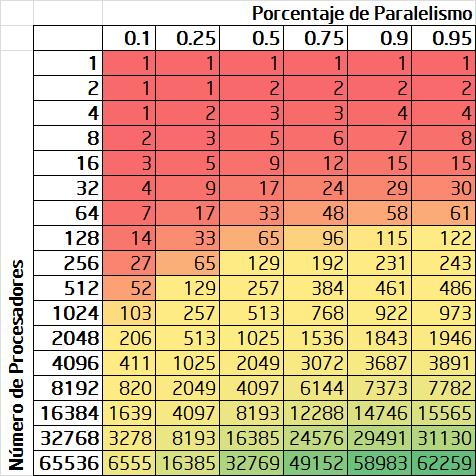
\includegraphics[width=7cm]{gustafson.png}
\caption{Tamaño de Datos de Entrada}
\label{fig:gustafson}
\end{center}
\end{figure}

Similarmente al cuadro anterior, podemos deducir de la figura \ref{fig:gustafson} que en el caso de un programa con sólo 10\% de paralelismo,
al incrementar los recursos 64x sólo podemos incrementar el tamaño del problema 7x. Sin embargo nos calcula
un incremento de 61x en el caso de tener 95\% de paralelismo.

\subsection{Métrica de {\it Karp-Flatt}}

Esta métrica es utilizada para medir el grado de paralelismo de una aplicación \cite{karp-flatt}.
Esta métrica nos permite rápidamente estimar la mejora posible al aplicar un alto nivel de paralelismo.

\bigskip

Dado un cómputo paralelo con una mejora de rendimiento $ \phi $ en $ P $
procesadores, donde $ P > 1 $. La fracción serial {\it Karp-Flatt}
representada con $ e $ y calculada según la ecuación \ref{eq:karp-flatt}
es determinada experimentalmente, mientras menor sea $ e $
mayor se supone el nivel de paralelismo posible.

\begin{eqnarray}
\label{eq:karp-flatt}
 e = \frac{\frac{1}{\psi} - \frac{1}{p}}{1 - \frac{1}{p}} 
\end{eqnarray}

Para un problema de tamaño fijo, la eficiencia típicamente disminuye cuando
el número de procesadores aumenta. Se puede entonces determinar si esta disminución
es debida a un paralelismo limitado, a un algoritmo no optimizado o un problema de
arquitectura del sistema.

\chapter{Herramientas de Soporte}

Este capítulo revisa las herramientas disponibles para soporte de análisis
de rendimiento de aplicaciones.

\section{Herramientas}

Se recomienda un proceso de aplicación gradual empezando por herramientas generales de alto nivel que analizan la aplicación como un todo; terminando con herramientas de bajo nivel que proveen detalles complejos de granularidad más fina en componentes particulares del sistema. Esto permite ir analizando el rendimiento sin tener que enfrentar la dificultad de un análisis complejo y extensivo desde un principio.

\begin{table}[H]
\caption{Aplicación Gradual de Herramientas}
\begin{tabular}{|l|l|} \hline
{\bf Característica} & {\bf Herramientas} \\ \hline
Capacidad del sistema & Benchmark HPCC \\ \hline
Medición de ejecución & {\tt time}, {\tt gettimeofday()}, {\tt MPI\_WTIME()} \\ \hline
Perfil de ejecución & {\tt gprof} \\ \hline
Comportamiento de la aplicación & {\tt gprof} \\ \hline
Comportamiento de librerías & valgrind, MPI vampir. \\ \hline
Comportamiento del sistema & oprofile \\ \hline
Vectorización & gcc \\ \hline
Contadores en {\it hardware} & oprofile, PAPI \\ \hline
\end{tabular}
\label{table:tools}
\end{table}

Primero se establece una línea de comparación al ejecutar una prueba de rendimiento del sistema, HPCC brinda un conjunto de métricas muy completo. Segundo se utilizan herramientas para medir el tiempo de ejecución de la aplicación sobre diferentes escenarios. time permite una ejecución directa sin modificación de código, {\tt gettimeofday()} requiere modificación de código pero puede ser utilizados con mayor libertad dentro de la aplicación.  
En el caso de estar utilizando la librería MPI {\tt MPI\_WTime()} y la herramienta VAMPIR\footnote{\tt http://www.vampir.eu/} proveen soporte especifico para análisis de rendimiento.
Tercero se dimensiona el comportamiento de la aplicación mediante un perfil de ejecución y un análisis de cuello de botella utilizando {\tt gprof}. Cuarto se analiza el comportamiento del sistema ejecutando la aplicación mediante {\tt oprofile}. Quinto se revisa el reporte del compilador para comprobar que se estén vectorizando los ciclos de cálculo más intensivos. Por último, se analiza el comportamiento de las unidades de cómputo utilizando soporte de {\it hardware} mediante herramientas como {\tt oprofile} y {\it Performance Application Programming Interface} (PAPI) \footnote{\tt http://icl.cs.utk.edu/papi/}.

\section{Tiempo de Ejecución}

time versus /usr/bin/time
gettimeofday() versus clock(3)

\subsection{Ejemplo: {\tt time(1)}}

\begin{lstlisting} 
$ /usr/bin/time -v ./program
Command being timed: "./program"
User time (seconds): 0.00
System time (seconds): 0.00
Percent of CPU this job got: 0%
Elapsed (wall clock) time (h:mm:ss or m:ss): 0:00.00
Average shared text size (kbytes): 0
Average unshared data size (kbytes): 0
Average stack size (kbytes): 0
Average total size (kbytes): 0
Maximum resident set size (kbytes): 3808
Average resident set size (kbytes): 0
Major (requiring I/O) page faults: 0
Minor (reclaiming a frame) page faults: 289
Voluntary context switches: 1
Involuntary context switches: 1
Swaps: 0
File system inputs: 0
File system outputs: 0
Socket messages sent: 0
Socket messages received: 0
Signals delivered: 0
Page size (bytes): 4096
Exit status: 0
\end{lstlisting}

\section{Perfil de Ejecución de Aplicación}

Estas herramientas denominadas {\it profilers} extraen el perfil dinámico de una aplicación en tiempo de ejecución. 
Se instrumenta la aplicación con una opción específica que incluye información de uso de las diferentes partes del programa y los recursos del sistema como por ejemplo procesador y memoria.

\bigskip

La aplicación debe ejecutarse con un conjunto de datos prefijado. El conjunto de
datos debe ser representativo y debe también ejercitar la aplicación por
una cantidad de tiempo suficiente como para intensificar el uso de los
recursos. Los datos del perfil de una ejecución son luego obtenidos en la
forma de un archivo de datos, luego se procede a procesar los datos acumulados
con un analizador respectivo.

\bigskip

Provee un perfil plano que consiste en una simple lista de las funciones
ejecutadas ordenadas por la cantidad acumulada de tiempo utilizado.
También provee el gráfico de llamadas anidadas, que muestra el tiempo
utilizado por cada función en llamadas sucesivas. Las funciones recursivas
son manejadas de manera especial ya que imposibilitan el armado de relaciones
de dependencias.

\subsection{Ejemplo: {\tt gprof}}

El perfil de ejecución muestra el tiempo individual y el tiempo acumulado en segundos de cada línea de código de la aplicación. Los binarios deben ser compilados con información extra de depuración, en el caso de {\tt gcc}, las opciones necesarias son {\tt -g -pg}. Si {\tt -g} no se encuentra presente entonces no se provee el reporte detallado por línea de ejecución. Esto permite identificar donde se esta gastando tiempo durante la ejecución.
La herramienta también muestra un cuadro de las llamadas entre funciones realizadas por el programa.
Esto permite visualizar el esquema de dependencias durante la ejecución.

\begin{lstlisting} 
$ gcc -g -pg program.c -o program
$ ./program
$ gprof program
...
\end{lstlisting}

\begin{lstlisting} 
Flat profile:
Each sample counts as 0.01 seconds.
% cumulative self self total
time seconds seconds calls us/call us/call name
37.50 0.15 0.15 48000 3.12 3.12 Life::neighbor_count(int, int)
...
\end{lstlisting}

\begin{lstlisting} 
Call graph
granularity: each sample hit covers 4 byte(s) for 2.50% of 0.40 seconds
index % time    self  children    called     name
      0.02 0.15 12/12 main [2]
[1] 42.5 0.02 0.15 12 Life::update(void) [1]
      0.15 0.00 48000/48000 Life::neighbor_count(int, int) [4]
--
          0.00    0.17       1/1           _start [3]
[2]     42.5    0.00    0.17       1         main [2]
          0.02    0.15      12/12          Life::update(void) [1]
          0.00    0.00      12/12          Life::print(void) [13]
          0.00    0.00      12/12          to_continue(void) [14]
          0.00    0.00       1/1           instructions(void) [16]
          0.00    0.00       1/1           Life::initialize(void) [15]
--
\end{lstlisting}

\section{Perfil de Ejecución de Sistema}

Un {\it profiler} a nivel de sistema analiza perfiles de rendimiento a nivel de núcleo del
sistema operativo. Actúa de forma transparente a nivel global. Utiliza
contadores de {\it hardware} del CPU e utiliza interrupciones de un temporizador
cuando no logra detectar soporte específico en {\it hardware}.

Para obtener realizar un análisis se necesita:

\begin{enumerate}
\item detener toda aplicación o servicio no relevante en el sistema.
\item ejecutar el profiler
\item ejecutar la aplicación
\item generar el resumen
\end{enumerate}

La herramienta de por si no se necesita acceder al código fuente de la aplicación.
Pero si esta disponible el código correspondiente se muestra anotado con contadores
si hay símbolos de depuración en el binario {\it debugging}.

Este método tiene en cuenta todos los componentes del sistema.
Se basa en la lectura de contadores del mismo procesador implementados en hardware.
Aunque tiene un costo adicional inherente, la sobrecarga es mínimo.

Los registros de {\it hardware} implementando contadores más utilizados son los
siguientes:

\begin{enumerate}
\item cantidad total de ciclos de procesador
\item cantidad total de instrucciones ejecutadas
\item cantidad de ciclos detenidos por espera de acceso a memoria
\item cantidad de instrucciones de punto flotante
\item cantidad de fallos de cache de nivel uno (L1)
\item cantidad de instrucciones de carga y descarga
\end{enumerate}

Las herramientas propietarias suelen tener acceso a contadores más específicos e
incluso programables para funciones determinadas de medición.

\subsection{Ejemplo: {\tt perf}}

En kernel más viejos que 2.6, oprofile \footnote{\tt http://oprofile.sourceforge.net/} sino perf \footnote{\tt https://perf.wiki.kernel.org}.

low overhead as they avoid system calls. una orden de magnitud al menos. mayor información.

\begin{lstlisting}
$ perf report
# Events: 1K cycles
# Overhead Command Shared Object Symbol
28.15% firefox-bin libxul.so [.] 0xd10b45
4.45% swapper  [kernel.kallsyms] [k] mwait_idle_with_hints
4.26% swapper  [kernel.kallsyms] [k] read_hpet
2.13% firefox-bin  firefox-bin [.] 0x1e3d
1.40% unity-panel-ser  libglib-2.0.so.0.2800.6 [.] 0x886f1
...
\end{lstlisting}

\begin{lstlisting}
 Percent |   Source code & Disassembly of program
         :   Disassembly of section .text:
         :   08048484 <main>:
         :   #include <string.h>
         :   #include <unistd.h>
         :   #include <sys/time.h>
         :
         :   int main(int argc, char **argv)
         :   {
    0.00 :    8048484:       55                      push   %ebp
    0.00 :    8048485:       89 e5                   mov    %esp,%ebp
...
    0.00 :    8048530:       eb 0b                   jmp    804853d <main+0xb9>
         :                           count++;
   14.22 :    8048532:       8b 44 24 2c             mov    0x2c(%esp),%eax
    0.00 :    8048536:       83 c0 01                add    $0x1,%eax
   14.78 :    8048539:       89 44 24 2c             mov    %eax,0x2c(%esp)
         :           memcpy(&tv_end, &tv_now, sizeof(tv_now));
         :           tv_end.tv_sec += strtol(argv[1], NULL, 10);
         :           while (tv_now.tv_sec < tv_end.tv_sec ||
         :                  tv_now.tv_usec < tv_end.tv_usec) {
         :                   count = 0;
         :                   while (count < 100000000UL)
   14.78 :    804853d:       8b 44 24 2c             mov    0x2c(%esp),%eax
   56.23 :    8048541:       3d ff e0 f5 05          cmp    $0x5f5e0ff,%eax
    0.00 :    8048546:       76 ea                   jbe    8048532 <main+0xae>
...
\end{lstlisting}

\begin{lstlisting}
perf stat -B dd if=/dev/zero of=/dev/null count=1000000

1000000+0 records in
1000000+0 records out
512000000 bytes (512 MB) copied, 0.956217 s, 535 MB/s

 Performance counter stats for 'dd if=/dev/zero of=/dev/null count=1000000':

            5,099 cache-misses             #      0.005 M/sec (scaled from 66.58%)
          235,384 cache-references         #      0.246 M/sec (scaled from 66.56%)
        9,281,660 branch-misses            #      3.858 %     (scaled from 33.50%)
      240,609,766 branches                 #    251.559 M/sec (scaled from 33.66%)
    1,403,561,257 instructions             #      0.679 IPC   (scaled from 50.23%)
    2,066,201,729 cycles                   #   2160.227 M/sec (scaled from 66.67%)
              217 page-faults              #      0.000 M/sec
                3 CPU-migrations           #      0.000 M/sec
               83 context-switches         #      0.000 M/sec
       956.474238 task-clock-msecs         #      0.999 CPUs

       0.957617512  seconds time elapsed
\end{lstlisting}

\section{Reporte de Vectorización}

Una herramienta de bajo nivel para analizar rendimiento es el mismo compilador
que debería estar vectorizando los ciclos de cómputo intensivo. Esto es muy
útil para detectar si los cuellos de botella ya se encuentran optimizados o no.

\begin{lstlisting}
$ gcc -c -O3 -ftree-vectorizer-verbose=1 ex.c
ex.c:7: note: LOOP VECTORIZED.
ex.c:3: note: vectorized 1 loops in function.
$ gcc -c -O3 -ftree-vectorizer-verbose=2 ex.c
ex.c:10: note: not vectorized: complicated access pattern.
ex.c:10: note: not vectorized: complicated access pattern.
ex.c:7: note: LOOP VECTORIZED.
ex.c:3: note: vectorized 1 loops in function.
$ gcc -c -O3 -fdump-tree-vect-details ex.c
...
\end{lstlisting}

No es posible vectorizar código recursivo, por lo que puede ser un buen punto a
optimizar. Por ejemplo en el caso de que el código sea recursivo se detalla lo siguiente:

\begin{lstlisting}
$ gcc -Wall -Wextra -O3 -ftree-vectorizer-verbose=4 -g queen.c
queen.c:22: note: vectorized 0 loops in function.
queen.c:35: note: vectorized 0 loops in function.
\end{lstlisting}

\chapter{Procedimiento de Análisis}

Este capítulo detalla las actividades necesarias para realizar análisis de rendimiento. También propone un procedimiento sistemático iterativo de aplicación de las actividades junto a la utilización de herramientas.

\section{Proceso}

\begin{figure}[H]
\label{fig:procedure}
\begin{center}
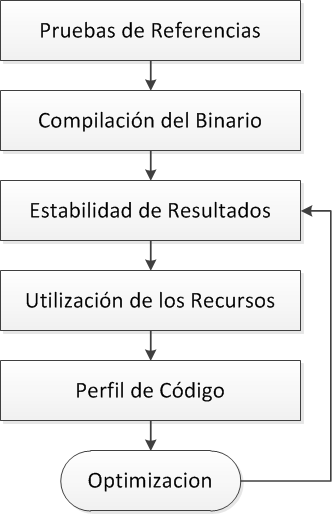
\includegraphics[width=5cm]{procedure.png}
\caption{Procedimiento de Análisis}
\end{center}
\end{figure}

\section{Paso a Paso}

\subsection{Pruebas de Referencia}

\begin{enumerate}
\item Ejecutar pruebas de rendimiento sobre el sistema a utilizar para poder entender sus capacidades máximas en contraste con las teóricas.

\begin{lstlisting}
$ pdsh -a hostname | sort | cut -f1 -d: > mpd.hosts
$ mpirun -n `wc -l mpd.hosts` ./hpcc
$ cat hpcout.inf
\end{lstlisting}

\begin{enumerate}
\item ¿Los resultados reflejan los esperados según las capacidades del sistema?
\item ¿Los FLOPS obtenidos se aproximan al rendimiento de un sistema similar o a la regla de $ CORES \times CLOCK \times FLOPS/CYCLE $ ?
\item ¿La latencia y ancho de banda de la red es la esperada?
\end{enumerate}

\item Comprobar variación de resultados para conocer la estabilidad de los mismos. La desviación estándar debe ser menor a 3 sigmas. Usar el promedio geométrico como referencia para comparaciones futuras.

\begin{lstlisting}
$ for i in `seq 1 32`; do /usr/bin/time -v ./app >> time.log; done
\end{lstlisting}

\begin{enumerate}
\item ¿ Son los resultados son reproducibles?
\item ¿ La desviación estándar es menor que 3?
\item ¿ Cuál es el promedio geométrico a ser usado en comparaciones futuras?
\end{enumerate}

\item Escalar tamaño del problema para calcular porcentaje de ejecución en paralelo.

\begin{lstlisting}
$ for size in `seq 1024 1024 10240`; do /usr/bin/time -v ./app $size >> size.log; done
\end{lstlisting}

\begin{enumerate}
\item ¿Cual es la relación entre el tiempo de las diferentes ejecuciones?
\item Es la relación lineal o constante?
\item Que porcentaje de la aplicación se estima paralelo?
\end{enumerate}

\item Escalar cantidad de procesadores para calcular cuanto se puede llegar a mejorar de acuerdo a leyes de {\it Amdalah} y {\it Gustafson}.

\begin{lstlisting}
$ for threads in `grep -c proc /proc/cpuinfo | xargs seq 1`; do OMP_NUM_THREADS=$threads ./app >> threads.log; done
\end{lstlisting}

\begin{lstlisting}
$ for nodes in `wc -l mpd.hosts | xargs seq 1`; do mpirun -n $nodes ./app >> nodes.log; done
\end{lstlisting}

\begin{enumerate}
\item ¿Cual es la relación entre el tiempo de las diferentes ejecuciones?
\item ¿Es la relación lineal o constante?
\end{enumerate}

\item Generar el perfil de llamadas a funciones dentro de la aplicación para revisar el diseño de la misma y los posibles cuellos de botella.

\begin{lstlisting}
$ gcc -g -pg app.c -o app
$ ./hpcc
\end{lstlisting}

\begin{lstlisting}
$ mpicc -g -pg app.c -o app
$ mpirun -n 30 ./app
\end{lstlisting}

\begin{lstlisting}
$ gprof --flat-profile --graph --annotated-source app
...
\end{lstlisting}

\begin{enumerate}
\item ¿Como esta diseñada la aplicación? ¿Que dependencias en librerías externas tiene?
\item ¿Implementa algún núcleo de computo conocido del tipo BLAS?
\item ¿Donde se concentra la mayor cantidad de tiempo de computo?
\end{enumerate}

\item utilizar el profiler a nivel de sistema

\item comprobar vectorizaciones

\begin{verbatim}
$ gcc -Wall -Wextra -O3 --report-loop
\end{verbatim}

\end{enumerate}

\chapter{Casos de Estudio}

Este capítulo aplica el modelo propuesto en el capítulo anterior. Varios ejemplos no triviales de aplicaciones de altas prestaciones son implementados
y analizados utilizando los benchmarks y herramientas anteriormente presentadas.

\section{Referencia}

Antes de empezar tomamos algunos datos de referencia del sistema utilizado.
Esto nos permite saber cuan lejos están nuestras aplicaciones de lo que se
puede obtener, también nos permite esbozar algunas hipótesis \ref{table:pruebas}.

\begin{table}[H]
    \caption{Hardware y software de cada nodo de cómputo}
    \centering
    \begin{tabular}{|l|l|}\hline
      {\bf Component} & {\bf Description} \\ \hline
      Server Board & Intel(R) S5000PAL \\ \hline
      CPU & Intel(R) Xeon(R) X5355 @ 2.66GHz \\ \hline
      Ethernet controller & Intel(R) 80003ES2LAN (Copper) (rev 01) \\ \hline
      RAM Memory & 4 GB DDR2 FB 667 MHz \\ \hline
      Operating System & Red Hat Enterprise 5.5 (Tikanga) \\ \hline
      Network Driver & Intel(R) PRO/1000 1.2.20-NAPI \\ \hline
      Ethernet Switch & Hewlett Packard HPJ4904A \\ \hline
    \end{tabular}
    \label{table:testbed}
\end{table}

\begin{table}[H]
\caption{Pruebas de Referencia}
  \begin{center}
    \begin{tabular}{|l|l|l|}\hline
      {\bf Benchmark} & {\bf Valor} & {\bf Unidad} \\ \hline
      dgemm & 70141 & mflops \\ \hline
      stream & 5931.6635 & MB/s \\ \hline
      hpl & 0.1217 & tflops \\ \hline
      ping pong BW & 1183.68 & MB/s \\ \hline
      ping ping latency & 4.49 & us \\ \hline
    \end{tabular}
    \end{center}
 \label{table:pruebas}
\end{table}

\begin{verbatim}
DGEMM, GFLOPS:   returned: '56.9715'
FFT, GFLOPS      returned: '2.43038'
HP Linpack, TFLOPS     returned: '0.057867'
PTRANS, GB/s     returned: '1.01094'
RandomAccess, GUPs/s    returned: '0.00417059'
Ring Bandwidth, GB/s     returned: '1.0678'
Ring Latency, us     returned: '3.68976'
STREAM Triad, GB/s   returned: '6.19899'
\end{verbatim}

\section{Multiplicación de Matrices}

La multiplicación de matrices es una operación fundamental en múltiples
campos de aplicación científica como la resolución de ecuaciones
lineales y la representación de grafos y espacios dimensionales. Por ello
existe abundante material sobre el tema.

{\small
\lstinputlisting{mm.c}
}

Diferentes alternativas de implementación son discutidas en
\cite{mm-matrixmultiplicationtool}.

\bigskip

El código fuente de una implementación simplista se encuentra adjuntado en
el apéndice. Al aplicar las herramientas vistas previamente se identifica
claramente que la multiplicación de los elementos de la matriz consume el
mayor tiempo de cómputo.

\bigskip

A continuación se muestra una comparación de diferentes métodos, se
demuestra claramente con este ejercicio la sofisticación de librerías
contra métodos artesanales de optimización.

\section{Distribución de Calor en Dos Dimensiones}

\begin{verbatim}
  for (j = 1; j < matrix_height - 1; j++) {
    for (i = 1; i < grid_length - 1; i++) {
      
      matrix[j * grid_length + i] = 
                     0.25 * (tmp[j * grid_length + i - 1]
                  + tmp[j * grid_length + i + 1]
                  + tmp[(j - 1) * grid_length + i]
                  + tmp[(j + 1) * grid_length + i]);

      diff = matrix[pos(i,j)] - tmp[pos(i,j)];

      if (error < diff) {
         error = diff;
      }
    }
  }
\end{verbatim}

La salida del cálculo puede graficarse fácilmente con {\it gnuplot}.

\begin{figure}[H]
\begin{center}
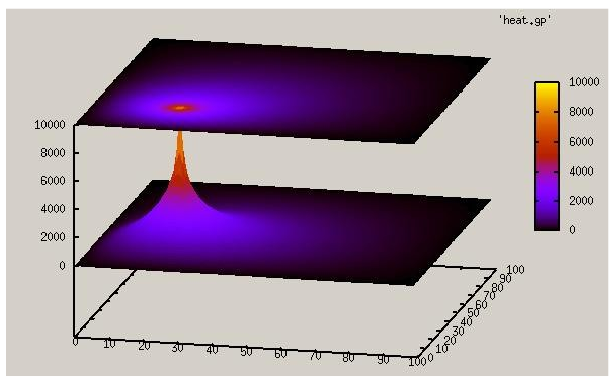
\includegraphics[width=10cm]{heat2d.png}
\caption{heat2d}
\end{center}
\end{figure}

\section{Problema de las Ocho Reinas}

El dilema trata en el problema de posicionar en un tablero de ajedrez ocho
reinas sin que alguna amenace a las demás. Una reina amenaza a cualquier otra
pieza en el tablero que este en la mismo diagonal, fila o columna.

\bigskip

Este problema suele resolverse utilizando recursión.

\begin{verbatim}
#include <stdio.h>
#include <stdlib.h>

static int *row = NULL;

static int available(int i, int n)
{
        int j = 1;
        while (row[i] != row[j] && abs(row[i] - row[j]) != (i - j) && j < n)
                j++;
        return ((i == j) ? 1 : 0);
}

static void show(int n)
{
        int i;
        for (i = 1; i <= n; i++)
                printf("row[\%d] = col[\%d]\n", i, row[i]);
}

static void queens(int i, int n)
{
        for (row[i] = 1; row[i] <= n; row[i]++) {
                if (available(i, n)) {
                        if (i == n) {
                                show(n);
                                exit(0);
                        } else
                                queens(i + 1, n);
                }
        }
}

int main()
{
        int n = atoi(getenv("QUEEN_N"));

        row = malloc(sizeof(int)*n);
        queens(1, n);
        show(n);

        return (0);
}
\end{verbatim}

\begin{verbatim}
Each sample counts as 0.01 seconds.
  \%   cumulative   self              self     total
 time   seconds   seconds    calls  ms/call  ms/call  name
 79.28      4.65     4.65                             available (queen.c:9 @ 400775)
  6.01      5.01     0.35                             queens (queen.c:24 @ 4008d3)
\end{verbatim}

Contrastando el tiempo requerido de ejecución entre la versión original y la instrumentada,
la diferencia fue 52.73 versus 49.61 segundos. Aproximadamente un 5.91 \%.

\begin{verbatim}
$ gcc -Wall -Wextra -O3 -g -pg queen.c
$ QUEEN\_N=30 time ./a.out
\end{verbatim}

\section{Transformadas de {\it Fourier}}

Una transformada de {\it Fourier} \cite{fourier} transforma una señal
digitalizada en una representación matemática de las frecuencias que la
componen. Su aplicación principal se da en problemas relacionados con la simulación del
movimiento de ondas como en la óptica y electromagnetismo. También se utiliza para el procesamiento de video y audio.

\bigskip

El código fuente de una implementación simplista de una aplicación que aplica una transformada de fourier a una fotografiá 
se encuentra adjuntado en el apéndice. Al aplicar las herramientas vistas previamente se identifica
claramente que la evaluación de derivadas parciales consume el mayor tiempo
de cómputo.

\bigskip

A continuación se muestra una comparación de diferentes métodos, se
demuestra claramente con este ejercicio la sofisticación de librerías
contra métodos artesanales de optimización. La siguiente es la versión
clásica de una implementación directa utilizando el algoritmo de
{\it Cooley-Tukey}.

\begin{verbatim}
int i, k;
float arg, sign = -1.0;

for (i = 0; i <= length/2; i++) {
    cosine[i] = sine[i] = 0.0;
    for (k = 0; k < length; k++) {
        arg = 2.0 * i * M_PI * k / length;
        sine[i] += input[k] * sign * sin(arg);
        cos[i] += input[k] * cos(arg);
    }
}
\end{verbatim}

\begin{verbatim}
int i;

for (i = 0; i <= length / 2; i++) {
    frequency[i] = 1.0 * i * rate / length;
    magnitude[i] =
        20.0 *
        log10( 2.0 * sqrt(sine[i] * sine[i] + cosine[i] * cosine[i]) /
        length);

    phase[i] = 180.0 * atan2(sine[i], cosine[i]) / M_PI - 90.0;
}
\end{verbatim}

Una implementación más eficiente es la denominada {\it Fast Fourier Transform}.
Un algoritmo aún más eficiente es el denominado {\it Goertzel}.

\bigskip

Este caso de aplicación no demuestra como al conocer el algoritmo implementado se
facilita la tarea de buscar algoritmos optimizados para cada caso en particular.

\chapter{Conclusiones}

Este trabajo aporta el estado del arte del análisis de rendimiento en
aplicaciones de cómputo de altas prestaciones. Discute, clasifica y detalla
diferentes opciones en herramientas de soporte. Se demuestra su aplicación
en varios problemas simples pero suficientemente interesantes. Propone un
proceso y un modelo simple de implementación para dimensionar las
optimizaciones posibles.

\bigskip

La optimización del rendimiento de una aplicación es algo no trivial, requiere de mucha
disciplina y del manejo de datos que identifiquen las partes a mejorar fehacientemente.
Existen diferentes niveles de abstracción en los cuales una aplicación puede ser analizada con el fin
de encontrar puntos de mejora. 

\bigskip

Es preciso realizar un análisis del comportamiento y del uso de los recursos antes de
empezar a optimizar una aplicación. Muchas veces las mejoras no son significativas si no
son realizadas en el lugar correcto.

\bigskip

El utilizar un mismo modelo para implementar las aplicaciones abre muchas puertas para
la automatización, comparación y estudio de técnicas de optimización que no pueden
ser siempre aplicadas sin reestructurar las aplicaciones.

\chapter{Trabajo Futuro}

\section{Infraestructura de Soporte para Análisis}

Este trabajo fue realizado como un primer paso a una implementación práctica del método propuesto,
incluyendo soporte automático para al utilización de las herramientas y la generación integrada de
reportes de análisis de rendimiento.

\section{Herramientas Adicionales de Soporte}

La implementación de nuevas tecnologías para el análisis de rendimiento
es incesante y continua, los siguientes proyectos están ampliamente
relacionados con este estudio.

\begin{itemize}
\item Proyecto A: descripción del proyecto A.
\item Proyecto B: descripción del proyecto B.
\item Proyecto C: descripción del proyecto C.
\end{itemize}

\section{Aplicación en el Mundo Real}

La utilización de estas ideas en una aplicación del mundo real es materia
pendiente, otra posibilidad es reimplementar desde cero alguna aplicación
científica en colaboración con algún grupo de investigación y realizar
varios ciclos de optimización.

\bigskip

Trabajo en conjunto con un algún grupo de investigación científica,
realizando análisis de rendimiento de aplicaciones ya existentes utilizadas
para publicación de resultados de modelado o simulación.

\section{Modelo en Etapas}

Luego de realizar este análisis se llego a la conclusión de que seria muy útil
el tener una infraestructura ya lista para prototipar rápidamente una aplicación.
La mayoría de los desarrolladores solo necesitan concentrarse en el algoritmo a
paralelizar y en la optimizacion de las etapas mas demandantes de cómputo.

\begin{thebibliography}{9}

\bibitem{mm-matrixmultiplicationtool}
  A. More,
  \emph{A Case Study on High Performance Matrix Multiplication},
  {\tt http://code.google.com/p/mm-matrixmultiplicationtool},
  2008.

\bibitem{parallel-programming}
  Paul E. McKenney,
  \emph{Is Parallel Programming Hard, And, If So, What Can You Do About It?},
  January, 2011.

\bibitem{fourier}
  J. B. Joseph Fourier, \emph{Théorie Analytique de la Chaleur}, Paris, 1822.

\bibitem{beowulf}
  T. Sterling, D. Savarese, D. J. Becker, J. E. Dorband, U. A. Ranawake,
  and C. V. Packer,
  \emph{Beowulf: A parallel workstation for scientific computation},
  1995.

\bibitem{mpi}
  Message Passing Interface Forum,
  \emph{MPI: A Message-Passing Interface Standard},
  2.2,
  2009.

\bibitem{openmp}
  OpenMP Architecture Review Board,
  \emph{OpenMP Application Program Interface}.
  3.0,
  2008.

\bibitem{tinetti}
  Fernando G Tinetti,
  \emph{Cómputo Paralelo en Redes Locales de Computadoras},
  2004.

\bibitem{gprof}
  Susan L. Graham,  Peter B. Kessler,  Marshall K. McKusick,
  \emph{gprof: A Call Graph Execution Profiler},
  1982.
  
\bibitem{oprofile}
  J. Levon,
  \emph{oprofile: hardware profiler for Linux systems},
       {\tt http://oprofile.sourceforge.net}.
  
\bibitem{hennessy-patterson}
  John. L. Hennesy, David A. Patterson,
  \emph{Computer Architecture: A Quantitative Approach, 3rd Edition},
  2002.

\bibitem{intel}
  Intel Press,
  \emph{Intel64 and IA-32 Architectures Software Developer's Manual - Volume
    3B: System Programming Guide, Part 2},
  March 2010.

\bibitem{what}
  Ulrich Deeper,
  \emph{What Every Programmer Should Know About Memory},
  November 2007.

\bibitem{patterns}
  G. Mattson, B.A. Sanders and B.L. Massingill, 
  \emph{Patterns for Parallel Programming, Addison-Wesley},
  2004.
  
\bibitem{automatic-performance-analysis}
  T. Margalef, J. Jorba, O. Morajko, A. Morajko, E. Luque,
  \emph{Different approaches to automatic performance analysis of distributed
    applications},
  2004.
  
\bibitem{capturing-performance-knowledge}
  K. Huck, O. Hernandez, V. Bui, S. Chandrasekaran, B. Chapman, A. Malony,
  L McInnes, B. Norris,
  \emph{Capturing performance knowledge for automated analysis},
  2008.
  
\bibitem{automatic-openmp-mpi-analysis}
  F. Wolf, B. Mohr,
  \emph{Automatic performance analysis of hybrid MPI/OpenMP applications},
  2003.
  
\bibitem{intro-software-performance}
  C. Smith,
  \emph{Introduction to software performance engineering: origins and
    outstanding problems},
  2007.

\bibitem{future-software-performance}
  M. Woodside, G. Franks, D. Petriu,
  \emph{The Future of Software Performance Engineering},
  2007.

\bibitem{critical-overview}
  J. Browne,
  \emph{A critical overview of computer performance evaluation},
  1976.

\bibitem{hpctoolkit}
  Rice University,
  \emph{HPC Toolkit}, {\tt http://hpctoolkit.org}.
       
\bibitem{papi}
  University of Tennessee,
  \emph{Performance Application Programming Interface},
       {\tt http://icl.cs.utk.edu/papi}.
       
\bibitem{amdahl}
  G. M. Amdahl,
  \emph{Validity of single-processor approach to achieving large-scale
    computing capability},
  Proceedings of AFIPS Conference, Reston, VA. 1967. pp. 483-485.
  
\bibitem{twelve-ways}
  D. Bailey, \emph{Twelve Ways to Fool the Masses When Giving Performance
    Results on Parallel Computers},
  RNR Technical Report, RNR-90-020, NASA Ames Research Center, 1991.
  
\bibitem{gustafson}
  J. L. Gustafson,
  \emph{Reevaluating Amdahl's Law}, CACM, 31(5), 1988. pp. 532-533.
  
\bibitem{karp-flatt}
  A. H. Karp and H. P. Flatt,
  \emph{Measuring Parallel Processor Performance},
  Communication of the ACM Volume 33 Number 5, May 1990.
  
\bibitem{myth}
  {Lee, Victor W. and Kim, Changkyu and Chhugani, Jatin and Deisher, Michael
    and Kim, Daehyun and Nguyen, Anthony D. and Satish, Nadathur and
    Smelyanskiy, Mikhail and Chennupaty}, Srinivas, and Hammarlund, Per and
  Singhal, Ronak and Dubey, Pradeep,
  \emph{Debunking the 100X GPU vs. CPU myth: an evaluation of throughput
    computing on CPU and GPU},
  2010.
  
\bibitem{stream}
  John D. McCalpin,
  \emph{A Survey of Memory Bandwidth and Machine Balance in Current High
    Performance Computers},
  1995.
  
\bibitem{counters}
  Dong H. Ahn and Jeffrey S. Vetter,
  \emph{Scalable Analysis Techniques for Microprocessor Performance Counter
    Metrics},
  2002.
  
\bibitem{linpack}
  J. Dongarra, J. Bunch, C. Moler and G. W. Stewart, 
  \emph{LINPACK Users Guide},
  1979.
  
\bibitem{hpl}
  A. Petitet, R. C. Whaley, J. Dongarra and A. Cleary, 
  \emph{HPL - A Portable Implementation of the High-Performance Linpack
    Benchmark for Distributed-Memory Computers}, {\tt http://www.netlib.org/benchmark/hpl}
  2008.

\bibitem{hpcc}
  Dongarra, J., Luszczek, P.,
  \emph{Introduction to the HPC Challenge Benchmark Suite}, ICL Technical Report,
  2005.  
  
\bibitem{gsl}
  Free Software Foundation (FSF), \emph{GNU Scientific Library (GSL)},
  {\tt http://www.gnu.org/software/gsl}.

\bibitem{latency}
	R. Garabato, A. More, V. Rosales,
	\emph{Optimizing Ethernet Latency in Beowulf Clusters},
	CLEI 2012.

\end{thebibliography}

\end{document}
